\documentclass[tikz,border=10pt]{standalone}
\begin{document}
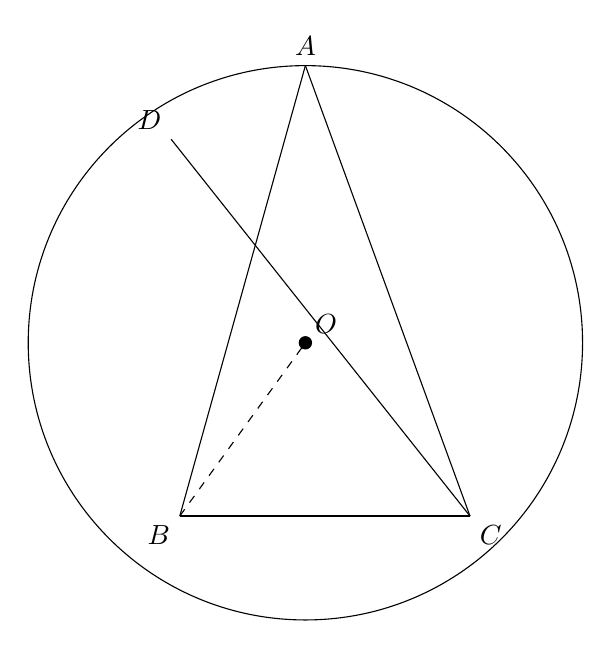
\begin{tikzpicture}[scale=1.1]

% Coordinates
\coordinate (O) at (0,0);
\coordinate (A) at (0,3.2);
\coordinate (B) at (-1.45,-2.0);
\coordinate (C) at (1.9,-2.0);
\coordinate (D) at (-1.55,2.35);

% Circle
\draw (O) circle [radius=3.2];

% Chords and segments
\draw (A) -- (B);
\draw (A) -- (C);
\draw (D) -- (C);
\draw (B) -- (C);
\draw[dashed] (B) -- (O);

% Point O
\fill (O) circle (2.2pt);

% Labels
\node[above] at (A) {$A$};
\node[below left] at (B) {$B$};
\node[below right] at (C) {$C$};
\node[above left] at (D) {$D$};
\node[above right] at (O) {$O$};

\end{tikzpicture}
\end{document}
